\let\negmedspace\undefined
\let\negthickspace\undefined
\documentclass[journal]{IEEEtran}
\usepackage[a5paper, margin=10mm, onecolumn]{geometry}
%\usepackage{lmodern} % Ensure lmodern is loaded for pdflatex
\usepackage{tfrupee} % Include tfrupee package

\setlength{\headheight}{1cm} % Set the height of the header box
\setlength{\headsep}{0mm}     % Set the distance between the header box and the top of the text

\usepackage{gvv-book}
\usepackage{gvv}
\usepackage{cite}
\usepackage{amsmath,amssymb,amsfonts,amsthm}
\usepackage{algorithmic}
\usepackage{graphicx}
\usepackage{textcomp}
\usepackage{xcolor}
\usepackage{txfonts}
\usepackage{listings}
\usepackage{enumitem}
\usepackage{mathtools}
\usepackage{gensymb}
\usepackage{comment}
\usepackage[breaklinks=true]{hyperref}
\usepackage{tkz-euclide} 
\usepackage{listings}
% \usepackage{gvv}                                        
\def\inputGnumericTable{}                                 
\usepackage[latin1]{inputenc}                                
\usepackage{color}                                            
\usepackage{array}                                            
\usepackage{longtable}                                       
\usepackage{calc}                                             
\usepackage{multirow}                                         
\usepackage{hhline}                                           
\usepackage{ifthen}                                           
\usepackage{lscape}


\renewcommand{\thefigure}{\theenumi}
\renewcommand{\thetable}{\theenumi}
\setlength{\intextsep}{10pt} % Space between text and floats

\numberwithin{equation}{enumi}
\numberwithin{figure}{enumi}
\renewcommand{\thetable}{\theenumi}	

% Marks the beginning of the document
\begin{document}
\bibliographystyle{IEEEtran}

\title{9-3-15}
\author{EE24BTECH11026-Srihaas Gunda}

% \maketitle
% \newpage
% \bigskip
{\let\newpage\relax\maketitle}

\textbf{QUESTION:} \\
	Find the area of the region \cbrak{\brak{x, y} : y^2 \leq 4x, 4x^2 + 4y^2 \leq 9}.\\
\textbf{SOLUTION:} \\
	\begin{table}[h!]    
		\centering
		\begin{tabular}[12pt]{ |c| c|}
    \hline
    \textbf{Variable} & \textbf{Description}\\ 
    \hline 
    $y^2 = 4x$ & Parabola\\
    \hline
    $4x^2 + 4y^2 = 9$ & Circle\\
    \hline
\end{tabular}

	\end{table}\\

	The general equation of a parabola with directrix $\vec{n}^{\top}\vec{x}=c$ is given by,
	\begin{align*}
		g\brak{\vec{x}}=\vec{x}^{\top}\vec{V}\vec{x}+2\vec{u}^{\top}\vec{x}+f=0\\
		\vec{V}=\norm{\vec{n}}^2\vec{I}-e^2\vec{n}\vec{n}^{\top}\\
		\vec{u}=ce^2\vec{n}-\norm{\vec{n}}^2\vec{F}\\
		f=\norm{\vec{n}}^2\norm{\vec{F}}^2-c^2e^2
	\end{align*}
	for the parabola $y^2=4x$, equation of directrix is, $\myvec{1&0}\vec{x}=-1$
	\begin{align*}
		\vec{V}&=\myvec{0&0\\0&1}\\
		\vec{u}&=\myvec{-2\\0}\\
		f&=0
	\end{align*}
	The given circle can be expressed as conics with parameters
	\begin{align*}
		\vec{V}&=\frac{1}{4}\myvec{9 & 0\\0 & 9}\\
		\vec{u}&=0\\
		f&=-\frac{81}{16}
	\end{align*}

	The intersection of two conics with parameters $\vec{V}_i,\vec{u}_i,f_i, i=1,2$ is defined as,
	\begin{align*}
		\vec{x}^{\top}\brak{\vec{V_1}+\mu\vec{V_2}}\vec{x}+2\brak{\vec{u_1}+\mu\vec{u_2}}^{\top}\vec{x}+\brak{f_1+\mu f_2}&=0\\
		\mu&=-\frac{4}{9}\\
	\end{align*} 
	On solving we get the points of intersection to be $\myvec{\frac{1}{2}\\\sqrt{2}}, \myvec{\frac{1}{2}\\-\sqrt{2}}$\\
	
	The desired area of region is given as\\
	\begin{align*}
		&= 2\sbrak{\int_{0}^{\frac{1}{2}} 2\sqrt{x} \, dx + \int_{\frac{1}{2}}^{\frac{3}{2}} \sqrt{\frac{9}{4}-x^2} \, dx}\\
		&= 2\sbrak{\frac{4}{3}\sqrt{x^3}}_0^\frac{1}{2} + 2\sbrak{\frac{x}{2}\sqrt{\frac{9}{4}-x^2} + \frac{9}{8}\sin^{-1}\brak{\frac{2x}{3}}}_\frac{1}{2}^\frac{3}{2}\\
		&= \frac{9\pi}{16}-\frac{1}{2\sqrt{2}}-\frac{9}{8}\sin^{-1}\brak{\frac{1}{3}}
	\end{align*}\\
	
\textbf{Computational Logic:} 
Using the trapezoidal rule to get the area. The trapezoidal rule is as follows.
\begin{align}
    \int^{b}_{a} f\brak{x}dx\approx \sum^{N}_{k=1}\frac{f\brak{x_{k+1}}+f\brak{x_{k}}}{2}h
\end{align}
where
\begin{align}
    h=\frac{b-a}{N}
\end{align}
$\therefore$The difference equation obtained is\\
\begin{align}
A = \int_a^b f\brak{x}\, dx \approx h\brak{\frac{1}{2}f\brak{a} + f\brak{x_1} + f\brak{x_2} \cdots + f\brak{x_{n-1}} + \frac{1}{2}f\brak{b}}\\
h = \frac{b-a}{n}\\
A = j_n, \text{ where, } j_{i + 1} = j_i + h\frac{f\brak{x_{i+1}} + f\brak{x_i}}{2}\\ 
\xrightarrow{} j_{i + 1} &= j_i + h\brak{{x_{i+1}^2}+{x_{i}^2}}\\
x_{i+1} &= x_i + h\\
\end{align}	
where,$a=0.5$ , $b=-0.5$ , $h=0.002$ ,taking $n=500$\\
\begin{align}
f(x) = \sqrt{\frac{9}{4} - x^2} - 2\sqrt{x}
\end{align}
Therefore, Required area =$3.0053$
	
	\begin{figure}[ht]
		\centering
		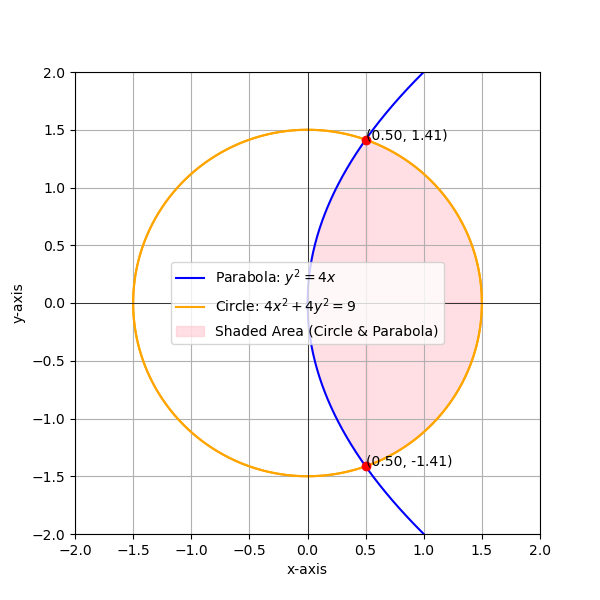
\includegraphics[width=0.8\textwidth]{figs/fig.png}
	\end{figure}
\end{document}
